\documentclass[11pt]{article}

\usepackage[margin=1in]{geometry}
\usepackage{amsmath,amssymb}
\usepackage{array}
\usepackage{booktabs}
\usepackage{microtype}
\usepackage{xcolor}
\usepackage{tikz}
\usepackage{pgfplots}
\usepackage[numbers,sort&compress]{natbib}
\usepackage[colorlinks=true,linkcolor=black,citecolor=black,urlcolor=black]{hyperref}
\pgfplotsset{compat=1.18}
\usetikzlibrary{positioning,arrows.meta,shapes.geometric}
\definecolor{lovegreen}{HTML}{1F7A76}
\definecolor{riskorange}{HTML}{D28B21}
\definecolor{lovepink}{HTML}{C0506F}
\definecolor{floorbrown}{HTML}{9B6A2F}
\definecolor{giveblue}{HTML}{4967A8}

\title{\textbf{The Love Integral}\\
\large A Reflexive Theory of Giving, Receiving, Deadweight Loss, and Relationship Risk}
\author{Joy Yang and Socrates Osorio}
\date{May 2026}

\newcommand{\Lfloor}{L_{\mathrm{floor}}}
\newcommand{\pcare}{\pi_{\mathrm{care}}}
\newcommand{\Risk}{\Omega}
\newcolumntype{L}[1]{>{\raggedright\arraybackslash}p{#1}}

\begin{document}
\maketitle

\begin{abstract}
This paper proposes that love is not merely an emotion, a preference, a sexual drive, or a moral posture, but a learned and reflexively self-modifying care function. A person $p$ loves a target $q$ when $p$ tracks $q$ through a trust-gated and floor-anchored evaluative process, treats $q$'s flourishing as a final end, identifies with $q$'s evaluative standpoint, and acts according to a policy whose divergence from genuine care is small. The default curve is receptive: how loved $p$ feels by $q$. This received-love curve is subjective and diagnostic; it is not by itself the whole normative definition of love. Love also has an outward curve: how much care $p$ gives to $q$. Costly giving that fails to become received love is deadweight loss, and love languages are the practical mechanism for minimizing it. Romantic love is the special case that adds sexual desire, pair-bonding substrates, negotiated exclusivity, and the construction of a durable ``we.'' We add a relationship-ending risk variable, $\Risk(t)$, because the possibility that the relationship ends is not merely another preference term: it is a structurally undesirable state that rises when love falls below reservation utility, anti-love pressure accumulates, trust fails, or dyadic imbalance becomes too large. The framework synthesizes recurring primitives from psychology, philosophy, and economics, and gives them a computational form suitable for empirical work and for an interactive dyadic visualizer.
\end{abstract}

\noindent\textbf{Keywords:} love, attachment, commitment, care, romantic love, relationship economics, trust, love languages, deadweight loss

\section{Introduction}
The ordinary word ``love'' compresses several phenomena that should not be collapsed: desire, attachment, robust concern, moral attention, commitment, market resistance, risk of loss, and the construction of a shared world. Psychology gives component models and attachment dynamics; philosophy gives the normative tests that distinguish love from fantasy or manipulation; economics explains why love is shaped by alternatives while also needing a floor that resists them.

The wager of this paper is that these traditions are not competitors. They are partial measurements of the same object. Love behaves like a learned function with inputs, weights, gates, floors, and update rules. A playful way to say the serious point is this: the love graph is not the relationship, but it lets us see what the relationship is doing.

The paper is written with two audiences in mind. For researchers, the model is explicit enough to test. For couples, the model is visual enough to answer ordinary questions: What makes my receiving curve go up? What pulls it down? What care am I giving? Is that care landing in the partner's receiving function? What protects the relationship from a bad week? What makes ending risk spike?

\begin{center}
\fbox{\begin{minipage}{.92\linewidth}
\textbf{Core claims.} (1) Romantic partner choice implicitly maximizes a lifetime love integral, not just current attraction. (2) Love has two coupled curves: received love and given care. (3) Love languages minimize deadweight loss between costly giving and felt receiving. (4) Compatibility lowers long-term risk by stabilizing trust, effort, and channel fit. (5) The desirable endpoint is not a permanent honeymoon spike, but a high stable plateau.
\end{minipage}}
\end{center}

\begin{table}[ht]
\centering
\small
\begin{tabular}{L{.14\linewidth}L{.28\linewidth}L{.24\linewidth}L{.22\linewidth}}
\toprule
Symbol & Plain meaning & Dashboard control/proxy & Why it matters \\
\midrule
$L^{rec}(t)$ & Love as felt by the receiver. & Love curve / integral. & Main subjective curve. \\
$G(t)$ & Care actively given outward. & Giving baseline, responsiveness, capacity. & Effort can be high even when received love is low. \\
$w_i$ & Receiver's channel weights. & Love-language weights. & Determines what counts as love. \\
$g(\tau)$ & Trust gate. & Trust and attachment style. & Controls whether care is registered. \\
$\Lfloor$ & Commitment floor. & Floor commitment. & Prevents short-run collapse. \\
$DWL$ & Deadweight loss between giving and receiving. & Deadweight loss / translation efficiency. & Measures wasted care. \\
$\Risk(t)$ & Relationship-ending risk pressure. & End-risk curve. & Captures fragility and downstream cost. \\
\bottomrule
\end{tabular}
\caption{Model map. The dashboard variables are intentionally aligned with the paper's primitives.}
\label{tab:model-map}
\end{table}

\begin{figure}[ht]
\centering
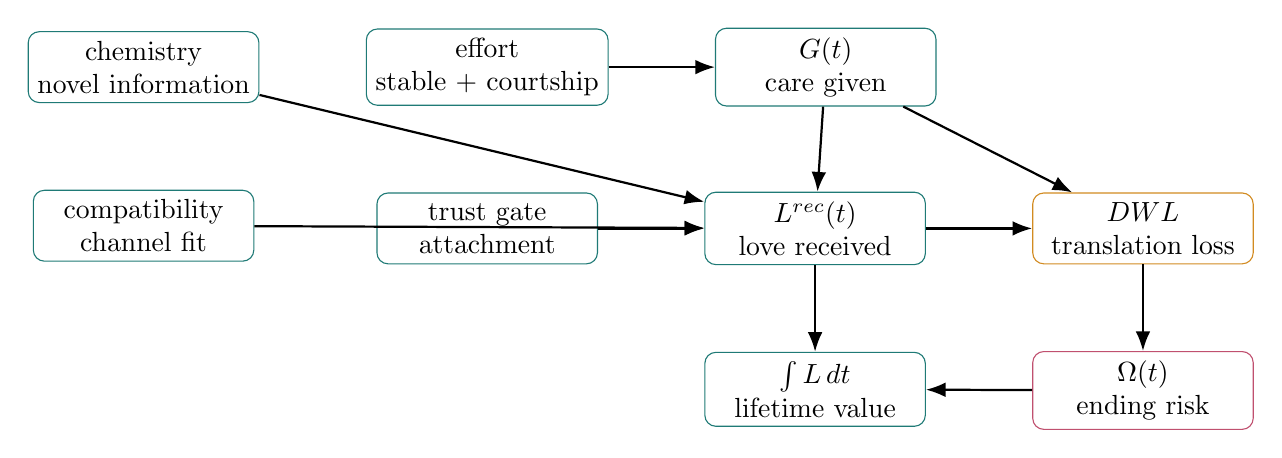
\begin{tikzpicture}[
  node distance=1.1cm and 1.35cm,
  box/.style={draw, rounded corners, align=center, minimum width=2.8cm, minimum height=.9cm, fill=white},
  good/.style={box, draw=lovegreen},
  warn/.style={box, draw=riskorange},
  bad/.style={box, draw=lovepink},
  arrow/.style={-{Latex[length=2.5mm]}, thick}
]
\node[good] (chem) {chemistry\\novel information};
\node[good, right=of chem] (effort) {effort\\stable + courtship};
\node[good, below=of chem] (fit) {compatibility\\channel fit};
\node[good, below=of effort] (trust) {trust gate\\attachment};
\node[good, right=of effort] (give) {$G(t)$\\care given};
\node[good, right=of trust] (receive) {$L^{rec}(t)$\\love received};
\node[warn, right=of receive] (dwl) {$DWL$\\translation loss};
\node[bad, below=of dwl] (risk) {$\Risk(t)$\\ending risk};
\node[good, below=of receive] (integral) {$\int L\,dt$\\lifetime value};
\draw[arrow] (chem) -- (receive);
\draw[arrow] (effort) -- (give);
\draw[arrow] (fit) -- (receive);
\draw[arrow] (trust) -- (receive);
\draw[arrow] (give) -- (receive);
\draw[arrow] (give) -- (dwl);
\draw[arrow] (receive) -- (dwl);
\draw[arrow] (dwl) -- (risk);
\draw[arrow] (receive) -- (integral);
\draw[arrow] (risk) -- (integral);
\end{tikzpicture}
\caption{Concept map. Chemistry and early effort create the initial rise; compatibility, trust, channel fit, and stable effort determine the plateau. Deadweight loss and ending risk subtract from the lifetime integral.}
\label{fig:concept-map}
\end{figure}

\section{Lifecycle Shape and Integral Maximization}
The first intuition should be the lifetime curve. Romantic love usually begins near zero, rises rapidly during the honeymoon stage, reaches an early peak, and then ideally converges to a stable near-horizontal line over the rest of the relationship. The early peak is not superficial. It contributes real area under the curve. This is one reason people prefer partners with chemistry over merely compatible strangers: chemistry steepens the early rise and raises the honeymoon peak, which increases the lifetime integral of love.

The honeymoon peak has two main sources. First, there is a lack-of-information term: learning a compatible, attractive person produces a strong feeling because every new detail is high-salience and can update the model of the beloved. Second, there is an unusually high effort term: early courtship contains extra dates, extra attention, surprise, grooming, wit, generosity, sexual novelty, and active impression management. Over time, the information term decays because the partner becomes known. The initial impression-effort term also usually decays. What remains is the stable effort trait: commitment, reliability, rituals, surprise, repair, and the couple's ordinary willingness to keep choosing each other. Couples with a high trait propensity to put in effort settle at a higher long-run plateau, which is extremely desirable because it dominates the lifetime integral.

A compact decomposition is:
\begin{equation}
L^{rec}(t)=\underbrace{P_{\mathrm{effort}}}_{\text{stable plateau}}+\underbrace{N_0e^{-\alpha t}}_{\text{novel information}}+\underbrace{E_0e^{-\beta t}}_{\text{impression effort}}-\underbrace{DWL(t)}_{\text{wasted care}}-\underbrace{X^-(t)}_{\text{anti-love}}.
\end{equation}
The desired long-run object is not a permanent honeymoon spike. It is a high plateau: a line that stays high because effort, compatibility, trust, and love-language fit continue to convert care into felt love.

The long-run plateau matters even more. A high honeymoon peak followed by collapse can produce less total love than a slightly lower peak that converges to a stable lifelong line. Compatibility is therefore not the same thing as chemistry, but it is highly correlated with long-term risk. Compatible partners have lower deadweight loss, lower anti-love activation, more stable trust, and lower ending risk. In integral terms, partner choice is partly an optimization problem:
\begin{equation}
q^*=\arg\max_q \int_0^T \left(L_{p,q}^{rec}(t)+G_{p\rightarrow q}(t)-c\Risk_{p,q}(t)-dDWL_{p,q}(t)\right)\,dt.
\end{equation}
The point is not that people explicitly run this calculation. The point is that chemistry, compatibility, risk, and love-language fit all affect the lifetime area.

\begin{figure}[ht]
\centering
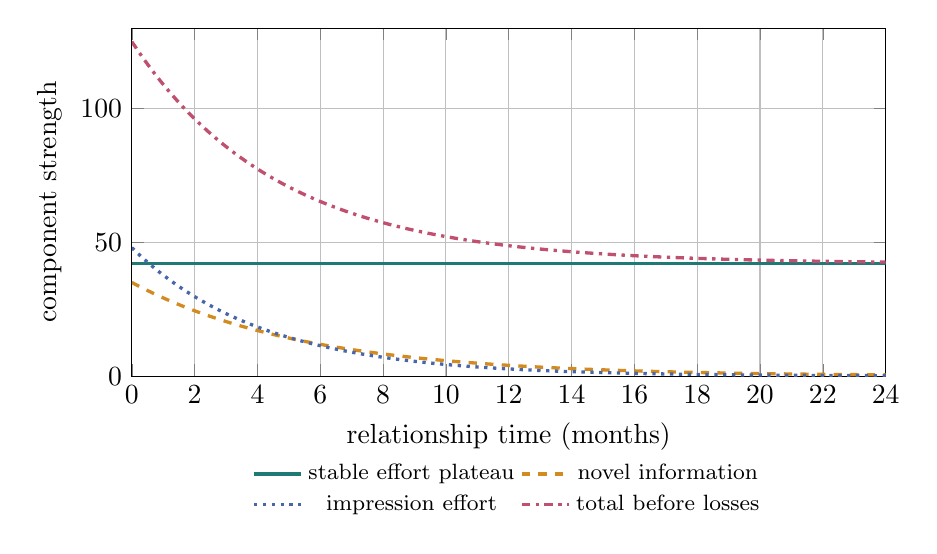
\begin{tikzpicture}
\begin{axis}[
  width=.92\linewidth,
  height=6cm,
  xlabel={relationship time (months)},
  ylabel={component strength},
  ymin=0,ymax=130,
  xmin=0,xmax=24,
  grid=both,
  legend style={at={(0.5,-0.22)},anchor=north,draw=none,fill=none,font=\footnotesize},
  legend columns=2,
]
\addplot[very thick,lovegreen,domain=0:24,samples=100] {42};
\addplot[very thick,riskorange,dashed,domain=0:24,samples=100] {35*exp(-0.18*x)};
\addplot[very thick,giveblue,dotted,domain=0:24,samples=100] {48*exp(-0.24*x)};
\addplot[very thick,lovepink,dash dot,domain=0:24,samples=100] {42+35*exp(-0.18*x)+48*exp(-0.24*x)};
\legend{stable effort plateau,novel information,impression effort,total before losses}
\end{axis}
\end{tikzpicture}
\caption{Mechanism of the honeymoon peak. Novel information decays as the partner becomes known. Impression effort usually declines from its courtship maximum. The long-run plateau is mostly determined by stable effort, commitment, repair, and the couple's willingness to keep creating novelty on purpose.}
\label{fig:honeymoon-components}
\end{figure}

\begin{figure}[ht]
\centering
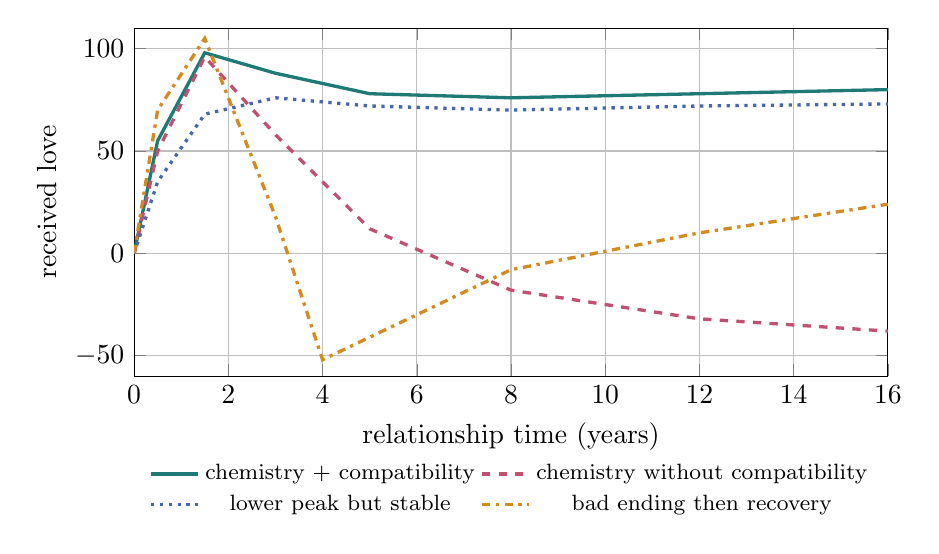
\begin{tikzpicture}
\begin{axis}[
  width=.92\linewidth,
  height=6cm,
  xlabel={relationship time (years)},
  ylabel={received love},
  ymin=-60,ymax=110,
  xmin=0,xmax=16,
  grid=both,
  legend style={at={(0.5,-0.22)},anchor=north,draw=none,fill=none,font=\footnotesize},
  legend columns=2,
]
\addplot[very thick,lovegreen] coordinates {(0,0) (0.5,55) (1.5,98) (3,88) (5,78) (8,76) (12,78) (16,80)};
\addplot[very thick,lovepink,dashed] coordinates {(0,0) (0.5,50) (1.5,96) (3,58) (5,12) (8,-18) (12,-32) (16,-38)};
\addplot[very thick,giveblue,dotted] coordinates {(0,0) (0.5,35) (1.5,68) (3,76) (5,72) (8,70) (12,72) (16,73)};
\addplot[very thick,riskorange,dash dot] coordinates {(0,0) (0.5,70) (1.5,105) (3,18) (4,-52) (6,-30) (8,-8) (12,10) (16,24)};
\legend{chemistry + compatibility,chemistry without compatibility,lower peak but stable,bad ending then recovery}
\end{axis}
\end{tikzpicture}
\caption{The lifetime integral explains why chemistry matters and why compatibility matters more over time. Chemistry creates the steep early rise and honeymoon peak. Compatibility lowers risk and lets the curve converge to a stable line rather than decay. If the relationship ends, the curve can fall to zero or below zero after a harmful ending, and the aftermath can lower future trust and future plateau capacity.}
\label{fig:lifecycle}
\end{figure}

If the relationship ends, the curve does not merely continue at the plateau. The directed romantic love curve for that relationship falls to zero, or below zero if the ending is experienced as betrayal, humiliation, or trauma. A bad ending can also alter future parameters: it can lower baseline trust, raise risk sensitivity, increase anti-love priors, and reduce giving capacity in later relationships. This is why the ending-risk variable matters even before the ending happens: high-risk love can have downstream costs beyond the present dyad.

\section{The Functional Core}
For person $p$ at time $t$, with target $q$ in relationship class $k$, let $\{\ell_i\}$ be a basis of care behaviors: attention, physical affection, reliability, words of recognition, instrumental help, sexual presence, forgiveness, intellectual engagement, protection, material provision, self-disclosure, and other channels. Let $x_i(t) \geq 0$ be the realized rate of behavior $\ell_i$ directed by $q$ to $p$, and let $w_i^{(p,k)}(t) \geq 0$ be $p$'s latent weight on that channel.

The instantaneous love function is:
\begin{equation}
L_p^{(k)}(t)=\max\left(\Lfloor^{(p,k)},\; g(\tau_p(t)) \sum_i w_i^{(p,k)}(t)x_i(t)+b_p^{(k)}\right).
\end{equation}

Here $g(\tau_p(t))\in[0,1]$ is a saturating trust gate, $b_p^{(k)}$ is a baseline, and $\Lfloor^{(p,k)}$ is a structural commitment level that survives short-run input shocks. The framework also requires reflexive updating:
\begin{equation}
w(t+1)=f(w(t),x(t),L_p(t),R_p^{(k)}(t),m_p(t)),
\end{equation}
where $R_p^{(k)}(t)$ is the relationship state and $m_p(t)$ is $p$'s outside-option market state. The point is not that every couple explicitly computes this equation. The point is that the equation organizes what the literatures repeatedly observe: people learn what care means, trust changes whether care is registered, and commitment places a lower bound on momentary volatility.

\subsection{Receiving and Giving Curves}
The curve above is the receiving curve: how loved $p$ feels by $q$. It is subjective registered love, not a claim that $q$ objectively loves $p$ exactly that much. It is the default curve because it is the one a person most directly experiences. But a full dyadic model also needs a giving curve:
\begin{equation}
G_{p\rightarrow q}(t)=h_p\left(L_{q\rightarrow p}^{\mathrm{rec}}(t),{\Lfloor}_p,\pi_p,\mathrm{capacity}_p,X_p^-(t)\right).
\end{equation}
The giving curve measures care sent outward by $p$ toward $q$. It is influenced by stable care identity, capacity, genuineness, and sometimes by reciprocity: many people give more easily when they feel loved, while mature love can preserve some giving even during temporary dips. This matters because $G_{p\rightarrow q}(t)$ is not automatically equal to $L_q^{\mathrm{rec}}(t)$. Care can be given in the wrong channel, at the wrong time, or under a policy the partner cannot register as care. A relationship can therefore fail in at least three ways: low receiving, low giving, or high translation loss between one person's giving and the other's receiving.

This translation loss is the relationship's deadweight loss of love. More precisely, deadweight loss is costly giving that is not converted into felt receiving:
\begin{equation}
DWL(t)=\max(0,G_{p\rightarrow q}(t)-L_q^{rec}(t))+\max(0,G_{q\rightarrow p}(t)-L_p^{rec}(t)).
\end{equation}
If received love is lower because the giver simply gave little, that is a deficit. If the giver gave a lot but the receiver did not feel loved in proportion to the cost, that is deadweight loss. Love languages are the practical technology for reducing this loss. If $q$'s high-weight channels are reliability and quality time, then $p$ can reduce $DWL$ by moving effort out of low-weight channels and into reliability and quality time. The goal is not to make everyone love identically; it is to route care through the channels where the partner's receiving function has the highest marginal response.

\subsection{Love Languages as Channel Optimization}
The phrase ``love language'' should be generalized beyond the familiar five categories. A love language is any channel $\ell_i$ for which the receiver has a high marginal response $w_i x_i(t)$ once trust permits the signal to enter. Traditional examples include words, gifts, acts of service, quality time, and touch. The broader basis also includes sex, cuddling, long conversations, intellectual collaboration, play, novelty, reliability, repair after conflict, public loyalty, shared silence, spiritual practice, ambition support, domestic competence, financial steadiness, humor, and respect for solitude.

The optimization problem is simple in form even when it is hard in life. Partner $p$ chooses an effort vector $e_{p\rightarrow q}$ subject to a budget and personal costs. Partner $q$ receives that effort through $q$'s weights and trust gate:
\begin{equation}
\max_{e_{p\rightarrow q}} \quad g_q(\tau_q)\sum_i w_i^q e_i - \sum_i c_i^p(e_i),
\end{equation}
where $c_i^p$ is the giver's cost of producing that channel. Deadweight loss appears when effort is placed in channels with low $w_i^q$ or high mistrust. Love-language knowledge is therefore information that moves the couple toward the Pareto frontier: more received love per unit of effort.

This also has a game-theoretic reading. In a one-shot interaction, each partner may underprovide costly care because effort is expensive and the return is uncertain. In a repeated relationship, stable trust and reciprocity can support a high-care equilibrium: I keep investing in your high-weight channels because you keep investing in mine, and because defection would lower future trust, receiving, and giving. Misread love languages create inefficient equilibria. Both partners can be exerting real effort while both feel under-loved.

\begin{table}[ht]
\centering
\small
\begin{tabular}{L{.18\linewidth}L{.23\linewidth}L{.23\linewidth}L{.20\linewidth}}
\toprule
Channel & High receiver value & Possible giver cost & Efficient move \\
\midrule
Cuddling & Receiver gets $+10$ from closeness and co-regulation. & Giver enjoys it only $+1$, or may feel touched-out. & Schedule bounded cuddling; use other touch when cost is high. \\
Sex & Receiver reads desire as primary romantic confirmation. & Giver may need more context, safety, or recovery time. & Treat sex as a high-weight channel, but protect consent and pacing. \\
Long conversations & Receiver feels known through depth and continuity. & Giver may find long processing draining. & Set intentional conversation windows rather than constant availability. \\
Reliability & Receiver treats consistency as proof of care. & Giver may value spontaneity and underestimate plan changes. & Make promises smaller and keep them; surprise inside stable boundaries. \\
Repair after conflict & Anxious receiver needs fast reassurance after rupture. & Avoidant giver may need time before re-engaging. & Agree on a repair protocol: pause, then return at a known time. \\
Novelty and play & Receiver needs self-expansion and aliveness. & Giver may prefer routine. & Put novelty on the calendar so it is not left to chance. \\
Solitude and space & Avoidant or overloaded receiver feels loved by non-intrusion. & Anxious giver may experience space as rejection. & Make space explicit and time-bounded so it does not read as abandonment. \\
\bottomrule
\end{tabular}
\caption{Love languages as efficiency channels. The target is not equal effort in every channel; it is high conversion from costly giving into felt receiving. Attachment style changes the weights and the perceived cost of the same act.}
\label{tab:language-optimization}
\end{table}

Attachment style changes both the weights and the trust gate. An anxious partner may assign very high weight to reassurance, fast repair, and consistency, while also having a volatile trust gate. An avoidant partner may assign high value to autonomy-respecting care and lower value to constant contact. A secure partner may have a broad receiving basis and a trust gate that recovers quickly after small ruptures. The same behavior can therefore be efficient in one dyad and inefficient in another. Ten minutes of cuddling can be a large positive transfer if one partner receives it strongly and the other experiences only mild cost; it can become inefficient or coercive if the giver experiences it as aversive. The correct solution is not to moralize the channel, but to solve the allocation problem with honesty about weights, costs, and trust.

\begin{figure}[ht]
\centering
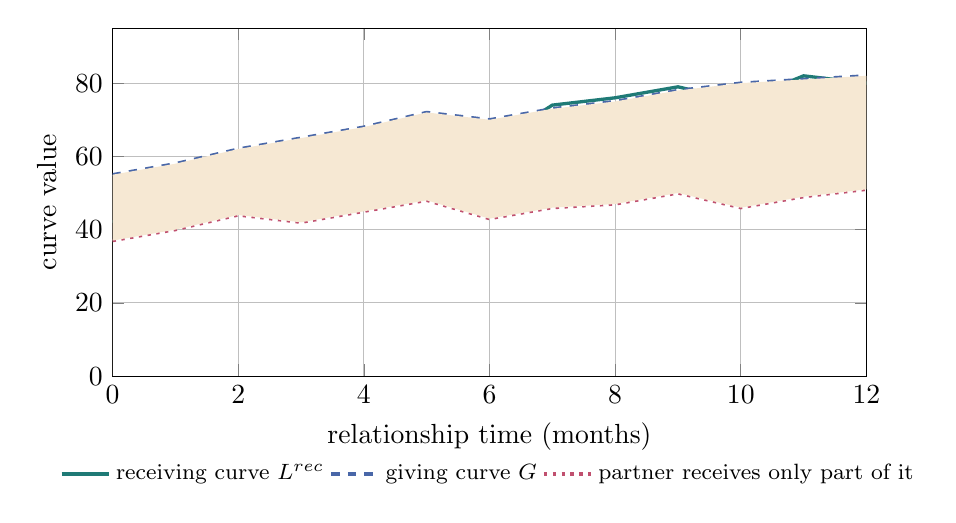
\begin{tikzpicture}
\begin{axis}[
  width=.92\linewidth,
  height=6cm,
  xlabel={relationship time (months)},
  ylabel={curve value},
  ymin=0,ymax=95,
  xmin=0,xmax=12,
  grid=both,
  legend style={at={(0.5,-0.22)},anchor=north,draw=none,fill=none,font=\footnotesize},
  legend columns=3,
]
\addplot[very thick,lovegreen] coordinates {(0,42) (1,54) (2,61) (3,57) (4,66) (5,70) (6,63) (7,74) (8,76) (9,79) (10,75) (11,82) (12,80)};
\addplot[very thick,giveblue,dashed] coordinates {(0,55) (1,58) (2,62) (3,65) (4,68) (5,72) (6,70) (7,73) (8,75) (9,78) (10,80) (11,81) (12,82)};
\addplot[very thick,lovepink,dotted] coordinates {(0,37) (1,40) (2,44) (3,42) (4,45) (5,48) (6,43) (7,46) (8,47) (9,50) (10,46) (11,49) (12,51)};
\addplot[fill=riskorange!20,draw=none] coordinates {(0,55) (1,58) (2,62) (3,65) (4,68) (5,72) (6,70) (7,73) (8,75) (9,78) (10,80) (11,81) (12,82) (12,51) (11,49) (10,46) (9,50) (8,47) (7,46) (6,43) (5,48) (4,45) (3,42) (2,44) (1,40) (0,37)} \closedcycle;
\legend{receiving curve $L^{rec}$,giving curve $G$,partner receives only part of it}
\end{axis}
\end{tikzpicture}
\caption{Giving and receiving are coupled but not identical. The shaded area is deadweight loss: effort that is given but not converted into felt love. Love languages minimize this area by aligning effort with high-weight receiving channels.}
\label{fig:giving-receiving}
\end{figure}

\begin{figure}[ht]
\centering
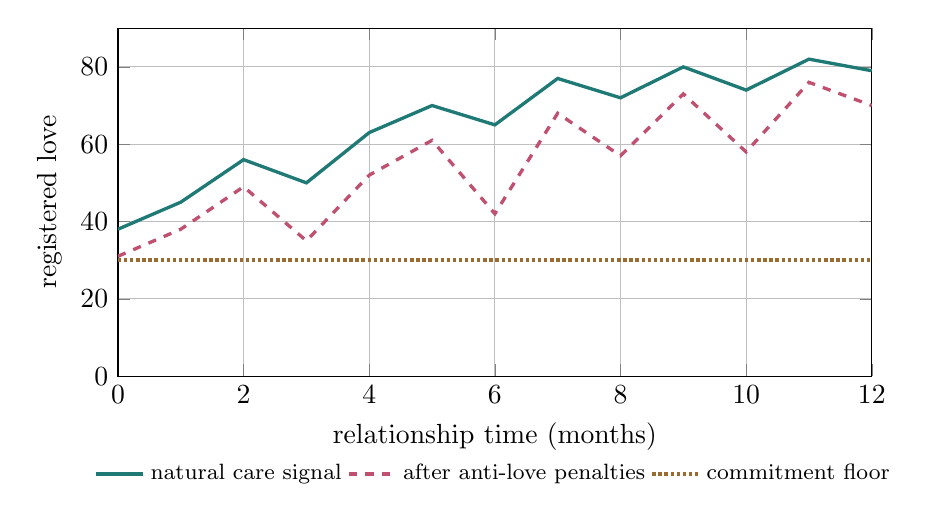
\begin{tikzpicture}
\begin{axis}[
  width=.92\linewidth,
  height=6cm,
  xlabel={relationship time (months)},
  ylabel={registered love},
  ymin=0,ymax=90,
  xmin=0,xmax=12,
  grid=both,
  legend style={at={(0.5,-0.22)},anchor=north,draw=none,fill=none,font=\footnotesize},
  legend columns=3,
]
\addplot[very thick,lovegreen] coordinates {(0,38) (1,45) (2,56) (3,50) (4,63) (5,70) (6,65) (7,77) (8,72) (9,80) (10,74) (11,82) (12,79)};
\addplot[very thick,lovepink,dashed] coordinates {(0,31) (1,38) (2,49) (3,35) (4,52) (5,61) (6,42) (7,68) (8,57) (9,73) (10,58) (11,76) (12,70)};
\addplot[very thick,floorbrown,densely dotted] coordinates {(0,30) (12,30)};
\legend{natural care signal,after anti-love penalties,commitment floor}
\end{axis}
\end{tikzpicture}
\caption{Anatomy of the curve. Positive channels create a natural care signal. Anti-love channels pull it down. The floor prevents brief shocks from becoming total collapse, but it does not erase the fact that the penalized signal has deteriorated.}
\label{fig:curve-anatomy}
\end{figure}

\section{Relationship-Ending Risk}
The possibility that the relationship ends should be modeled directly, before we talk about secondary refinements. Let $\Risk_p(t)\in[0,1]$ be $p$'s relationship-ending risk pressure. It is undesirable in itself because a breakup is not just a lower instantaneous love score; it is a transition into a different state with emotional, practical, social, and identity costs. The following expression is schematic rather than empirically calibrated:
\begin{equation}
\Risk_p(t)=\sigma\left(\eta_p\left[R_p(t)-L_p(t)+\lambda X_p^-(t)+\mu(1-g(\tau_p(t)))+\nu m_p(t)-\kappa {\Lfloor}_p\right]\right),
\end{equation}
where $\sigma$ is a logistic function, $\eta_p$ is risk sensitivity, $R_p(t)-L_p(t)$ is the deficit below reservation utility, $X_p^-(t)$ is anti-love pressure, low trust raises risk, visible outside options raise risk, and the floor partially protects against ending. The sign matters: love is desirable; ending risk is not. A relationship can have high love and high risk if the curve is intense but unstable.

\begin{figure}[ht]
\centering
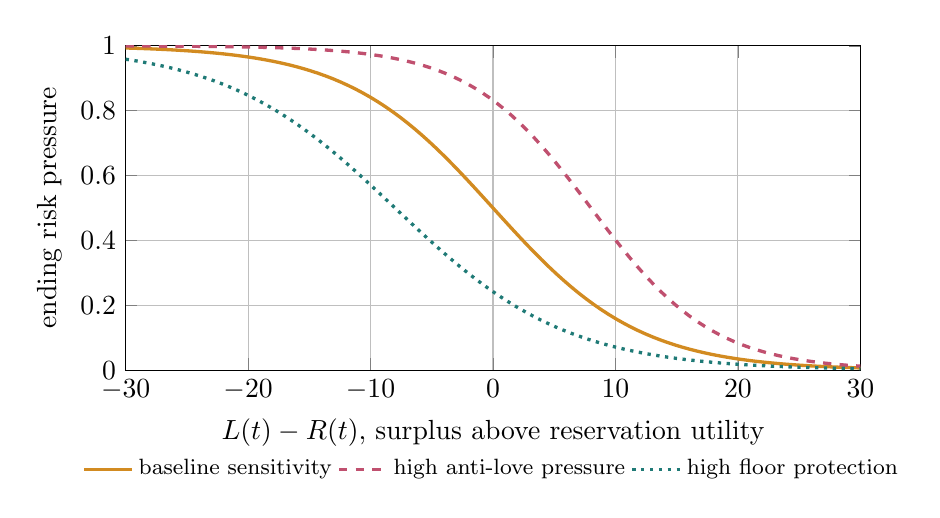
\begin{tikzpicture}
\begin{axis}[
  width=.9\linewidth,
  height=5.7cm,
  xlabel={$L(t)-R(t)$, surplus above reservation utility},
  ylabel={ending risk pressure},
  ymin=0,ymax=1,
  xmin=-30,xmax=30,
  grid=both,
  legend style={at={(0.5,-0.24)},anchor=north,draw=none,fill=none,font=\footnotesize},
  legend columns=3,
]
\addplot[very thick,riskorange,domain=-30:30,samples=100] {1/(1+exp((x-0)/6))};
\addplot[very thick,lovepink,dashed,domain=-30:30,samples=100] {1/(1+exp((x-8)/5))};
\addplot[very thick,lovegreen,dotted,domain=-30:30,samples=100] {1/(1+exp((x+8)/7))};
\legend{baseline sensitivity,high anti-love pressure,high floor protection}
\end{axis}
\end{tikzpicture}
\caption{Risk is easiest to understand as a surplus problem. When registered love falls below reservation utility, ending risk rises. Anti-love shifts the risk curve rightward, so more surplus is needed to feel safe; floor commitment shifts it leftward, so the dyad can absorb more ordinary volatility.}
\label{fig:risk}
\end{figure}

\section{Genuineness and Anti-Love}
Observable care can be faked. A policy can emit the right signals while optimizing for control, reward, or reputation. To exclude Goodhart-style pseudo-love, the behavioral policy $\pi_p$ must stay close to a pure-care policy:
\begin{equation}
D_{\mathrm{KL}}(\pi_p \| \pcare(q)) \leq \epsilon.
\end{equation}
This condition captures the difference between affection and manipulation, between autonomous care and controlled performance, and between seeing the beloved and projecting onto them.

The visualizer operationalizes a related distinction between love languages and anti-love languages. Positive channels raise the natural curve. Anti-love channels, such as contempt, unreliability, humiliation, or chronic withdrawal, subtract from it. Their absence does not create bonus love; it only removes a penalty:
\begin{align}
L_{\mathrm{natural}}(t) &= g(\tau(t)) X^+(t)+b,\\
L_{\mathrm{penalized}}(t) &= L_{\mathrm{natural}}(t)-X^-(t),\\
L(t)&=\max(\Lfloor,L_{\mathrm{penalized}}(t)).
\end{align}

\begin{figure}[ht]
\centering
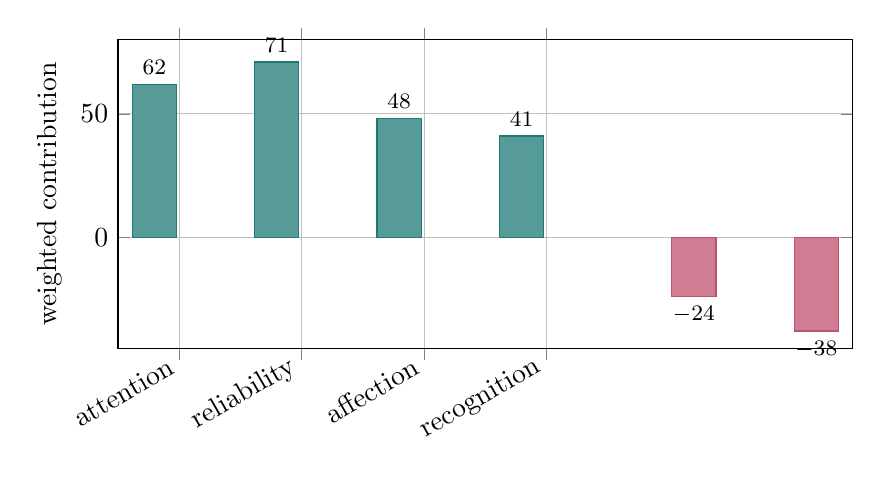
\begin{tikzpicture}
\begin{axis}[
  width=.9\linewidth,
  height=5.5cm,
  ybar,
  bar width=16pt,
  symbolic x coords={attention,reliability,affection,recognition,withdrawal,contempt},
  xtick=data,
  x tick label style={rotate=30,anchor=east},
  ylabel={weighted contribution},
  ymin=-45,ymax=80,
  grid=major,
  nodes near coords,
  every node near coord/.append style={font=\footnotesize},
]
\addplot[fill=lovegreen!75,draw=lovegreen] coordinates {(attention,62) (reliability,71) (affection,48) (recognition,41)};
\addplot[fill=lovepink!75,draw=lovepink] coordinates {(withdrawal,-24) (contempt,-38)};
\end{axis}
\end{tikzpicture}
\caption{Love languages and anti-love languages are not symmetric goods. More attention, reliability, affection, and recognition can lift the curve; less contempt does not create surplus love, it removes damage.}
\label{fig:channels}
\end{figure}

\section{Definition}
A directed care relation from $p$ to $q$ exhibits love over a relevant window $W$ if the following conditions obtain:

\begin{enumerate}
\item \textbf{Robust concern:} $p$ has a stable, behaviorally expressed disposition that $q$ flourish.
\item \textbf{Reflexive care function:} $p$ maintains a trust-gated, weighted, floor-anchored evaluative function.
\item \textbf{Floor commitment:} $\Lfloor$ is above a purely market-derived reservation utility.
\item \textbf{Two-curve structure:} love has a receptive curve $L^{rec}$ and a giving curve $G$; mature dyadic love requires both, plus enough channel fit for giving to be received.
\item \textbf{Identification:} $q$'s flourishing enters $p$'s evaluative perspective as partly constitutive of $p$'s own.
\item \textbf{Genuineness:} $\pi_p$ remains close to $\pcare(q)$.
\item \textbf{Accurate attention:} $p$'s model of $q$ tracks dimensions that matter to $q$.
\item \textbf{Reflexivity:} $p$'s weights update in response to joint history and $q$'s actual flourishing.
\item \textbf{Risk accounting:} $p$'s relationship-ending risk $\Risk_p(t)$ is tracked as a separate undesirable state variable, not confused with low love itself.
\end{enumerate}

Romantic love adds sexual desire, pair-bonding substrates, an exclusivity norm or negotiated equivalent, a constructive ``we,'' and heightened non-substitutability.

\section{Dyadic Imbalance}
For a couple, each partner has two directed curves: a receiving curve and a giving curve. The receiving integral
\begin{equation}
\mathcal{I}_p^{rec}=\int_{0}^{T} L_p^{rec}(t)\,dt
\end{equation}
measures cumulative received love as registered by $p$ under $p$'s weights, trust, and floor. The giving integral
\begin{equation}
\mathcal{I}_{p\rightarrow q}^{give}=\int_{0}^{T} G_{p\rightarrow q}(t)\,dt
\end{equation}
measures cumulative care sent by $p$ toward $q$. A dyad can then be described by a total received-love integral,
\begin{equation}
\mathcal{I}_{\mathrm{total}}^{rec}=\mathcal{I}_p^{rec}+\mathcal{I}_q^{rec},
\end{equation}
and an imbalance gap,
\begin{equation}
\Delta^{rec}=\left|\mathcal{I}_p^{rec}-\mathcal{I}_q^{rec}\right|.
\end{equation}
The Threshold for Maximum Tolerance of Imbalance is a chosen value $\Theta$ such that the relationship becomes structurally strained when $\Delta^{rec}>\Theta$. This is not a verdict on whether the couple should stay together. It is a diagnostic: a gap above $\Theta$ means the dyad is asking one person to carry more cumulative love load than the current model says is tolerable.

A second diagnostic is deadweight loss:
\begin{equation}
DWL=\max(0,\mathcal{I}_{p\rightarrow q}^{give}-\mathcal{I}_q^{rec})+\max(0,\mathcal{I}_{q\rightarrow p}^{give}-\mathcal{I}_p^{rec}).
\end{equation}
Low $DWL$ means the care each partner sends is broadly landing in the other's receiving curve. High $DWL$ means someone may be giving a lot, but the partner is not feeling loved in proportion to that effort. A separate under-provision deficit should be tracked when giving itself is low. Love languages minimize $DWL$ by identifying which channels have high marginal return in the receiver's curve.

Risk also has a dyadic component. Let
\begin{equation}
\Risk_{\mathrm{dyad}}(t)=\frac{\Risk_p(t)+\Risk_q(t)}{2}+\chi\max(0,\Delta^{rec}(t)-\Theta)+\zeta DWL(t),
\end{equation}
where $\chi$ converts excess receiving imbalance into additional ending risk and $\zeta$ converts translation loss into risk. This captures a common pattern: each partner may be trying, yet the relationship still becomes fragile because care is not landing where the other person's weights are highest.

\begin{figure}[ht]
\centering
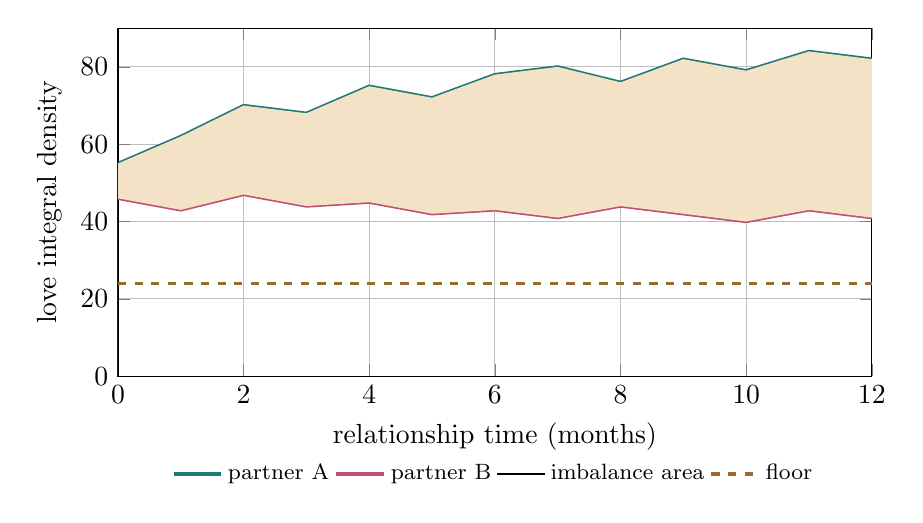
\begin{tikzpicture}
\begin{axis}[
  width=.92\linewidth,
  height=6cm,
  xlabel={relationship time (months)},
  ylabel={love integral density},
  ymin=0,ymax=90,
  xmin=0,xmax=12,
  grid=both,
  legend style={at={(0.5,-0.22)},anchor=north,draw=none,fill=none,font=\footnotesize},
  legend columns=4,
]
\addplot[very thick,lovegreen] coordinates {(0,55) (1,62) (2,70) (3,68) (4,75) (5,72) (6,78) (7,80) (8,76) (9,82) (10,79) (11,84) (12,82)};
\addplot[very thick,lovepink] coordinates {(0,46) (1,43) (2,47) (3,44) (4,45) (5,42) (6,43) (7,41) (8,44) (9,42) (10,40) (11,43) (12,41)};
\addplot[fill=riskorange!25,draw=none] coordinates {(0,55) (1,62) (2,70) (3,68) (4,75) (5,72) (6,78) (7,80) (8,76) (9,82) (10,79) (11,84) (12,82) (12,41) (11,43) (10,40) (9,42) (8,44) (7,41) (6,43) (5,42) (4,45) (3,44) (2,47) (1,43) (0,46)} \closedcycle;
\addplot[very thick,floorbrown,dashed] coordinates {(0,24) (12,24)};
\legend{partner A,partner B,imbalance area,floor}
\end{axis}
\end{tikzpicture}
\caption{The imbalance area is the visual version of $\Delta^{rec}$. Even when both receiving curves stay above the floor, a persistent gap can produce resentment, fatigue, or ending risk.}
\label{fig:imbalance}
\end{figure}

\section{Case Study: Maya and Leo}
Consider Maya and Leo. Maya registers love most strongly through reliability, quality time, and words of recognition. Her anti-love channels are last-minute cancellation and contempt during conflict. Leo registers love through physical affection, playful novelty, and practical help. His anti-love channels are emotional distance and public criticism. Both people love each other, but their graphs can still diverge because the same behavior has different weights.

\begin{table}[ht]
\centering
\begin{tabular}{lrrr}
\toprule
Channel & Maya's weight & Leo's weight & Interpretation \\
\midrule
Reliability & 1.50 & 0.80 & Very high for Maya; moderate for Leo \\
Quality time & 1.35 & 1.00 & High for both \\
Words of recognition & 1.10 & 0.70 & Maya hears love verbally \\
Physical affection & 0.80 & 1.45 & Leo hears love bodily \\
Play and novelty & 0.65 & 1.30 & Leo needs re-expansion energy \\
Practical help & 0.90 & 1.15 & Useful but not sufficient alone \\
Cancellation & -1.25 & -0.70 & Maya treats it as reliability damage \\
Emotional distance & -0.75 & -1.20 & Leo treats it as attachment damage \\
\bottomrule
\end{tabular}
\caption{A simple channel map. The numbers are not moral scores; they are weights. A partner can be trying hard and still miss the channel with the highest weight.}
\label{tab:case-weights}
\end{table}

Imagine Leo plans elaborate dates but often changes plans at the last minute. His giving curve may be high: he is investing effort, novelty, and planning. But Maya receives the novelty through a medium that also triggers a reliability penalty, so her receiving curve rises and then gets pulled down. Imagine Maya responds by becoming less physically affectionate while still doing practical favors. Her giving curve also stays nonzero, but Leo receives help while his highest-weight channel is not being fed, and his anti-love channel of distance starts to activate. Neither partner is necessarily uncaring. The problem is that their giving curves are not landing cleanly in the other's receiving function.

\begin{table}[ht]
\centering
\small
\begin{tabular}{rL{.21\linewidth}L{.30\linewidth}L{.28\linewidth}}
\toprule
Week & Event & Curve movement & Interpretation \\
\midrule
0 & First connection & Both receiving curves start well above zero. & Chemistry creates a steep early slope. \\
1 & Long date, high attention & Maya rises; Leo's giving rises. & Quality time feeds both partners. \\
2 & Leo reschedules twice & Maya drops from reliability damage. & High giving in novelty is partly wasted by cancellation. \\
3 & Repair conversation & Maya rebounds; risk falls. & Words plus reliability repair lower deadweight loss. \\
4 & Maya gets busy and less affectionate & Leo drops. & Practical help does not fully substitute for affection. \\
5--6 & Both try harder in their own default styles & Giving remains high, receiving stays low. & This is the deadweight-loss zone. Effort is real, but poorly translated. \\
7 & They identify top channels explicitly & Both receiving curves recover. & Love languages redirect effort to high-marginal-return channels. \\
10 & New stable routine & Curves approach a flatter line. & Compatibility lowers long-run risk and stabilizes the integral. \\
\bottomrule
\end{tabular}
\caption{What is happening at the major points in Figure~\ref{fig:case-study}. The graph is not a generic mood trend; each bend corresponds to a channel-specific event.}
\label{tab:case-timeline}
\end{table}

\begin{figure}[ht]
\centering
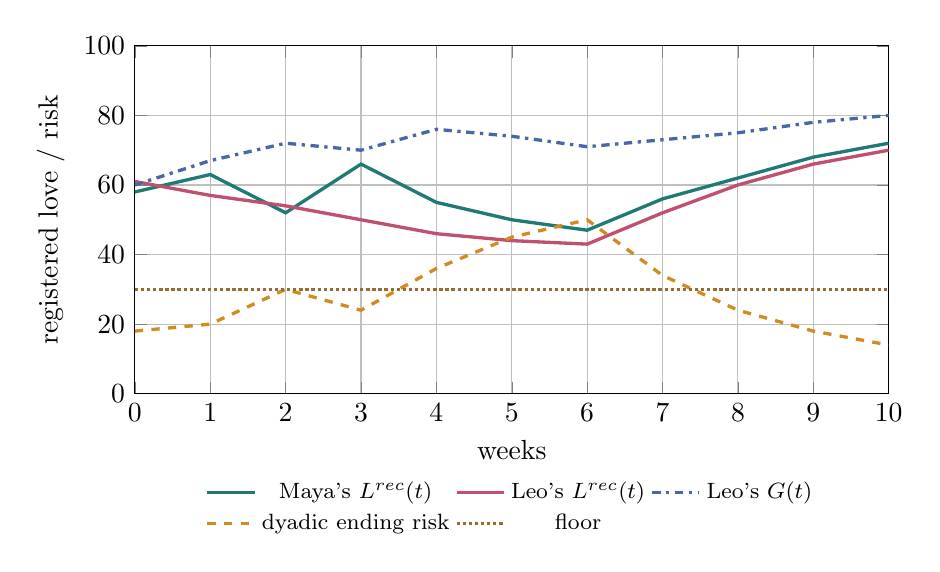
\begin{tikzpicture}
\begin{axis}[
  width=.92\linewidth,
  height=6cm,
  xlabel={weeks},
  ylabel={registered love / risk},
  ymin=0,ymax=100,
  xmin=0,xmax=10,
  grid=both,
  legend style={at={(0.5,-0.22)},anchor=north,draw=none,fill=none,font=\footnotesize},
  legend columns=3,
]
\addplot[very thick,lovegreen] coordinates {(0,58) (1,63) (2,52) (3,66) (4,55) (5,50) (6,47) (7,56) (8,62) (9,68) (10,72)};
\addplot[very thick,lovepink] coordinates {(0,61) (1,57) (2,54) (3,50) (4,46) (5,44) (6,43) (7,52) (8,60) (9,66) (10,70)};
\addplot[very thick,giveblue,dash dot] coordinates {(0,60) (1,67) (2,72) (3,70) (4,76) (5,74) (6,71) (7,73) (8,75) (9,78) (10,80)};
\addplot[very thick,riskorange,dashed] coordinates {(0,18) (1,20) (2,30) (3,24) (4,36) (5,45) (6,50) (7,34) (8,24) (9,18) (10,14)};
\addplot[very thick,floorbrown,densely dotted] coordinates {(0,30) (10,30)};
\legend{Maya's $L^{rec}(t)$,Leo's $L^{rec}(t)$,Leo's $G(t)$,dyadic ending risk,floor}
\end{axis}
\end{tikzpicture}
\caption{In the case study, week 6 is the danger point. Leo's giving remains high, but enough of it misses Maya's reliability-weighted receiving curve that anti-love and mismatch push ending risk upward. Repair starts when each partner feeds the other's high-weight channels.}
\label{fig:case-study}
\end{figure}

The repair is intuitive. Leo does not need to become a different person; he needs to make reliability less noisy because Maya's model treats plan stability as evidence of care. Maya does not need to perform constant affection; she needs to know that Leo's curve treats affectionate contact as a primary attachment channel, not a decorative extra. The theory is useful only if it helps a couple find this level of translation.

\begin{figure}[ht]
\centering
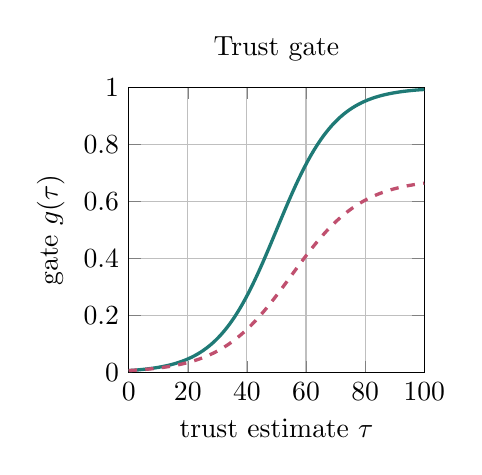
\begin{tikzpicture}
\begin{axis}[
  width=.44\linewidth,
  height=5.2cm,
  xlabel={trust estimate $\tau$},
  ylabel={gate $g(\tau)$},
  ymin=0,ymax=1,
  xmin=0,xmax=100,
  grid=both,
  title={Trust gate},
]
\addplot[very thick,lovegreen,domain=0:100,samples=100] {1/(1+exp(-(x-50)/10))};
\addplot[very thick,lovepink,dashed,domain=0:100,samples=100] {0.68/(1+exp(-(x-55)/12))};
\end{axis}
\end{tikzpicture}
\hfill
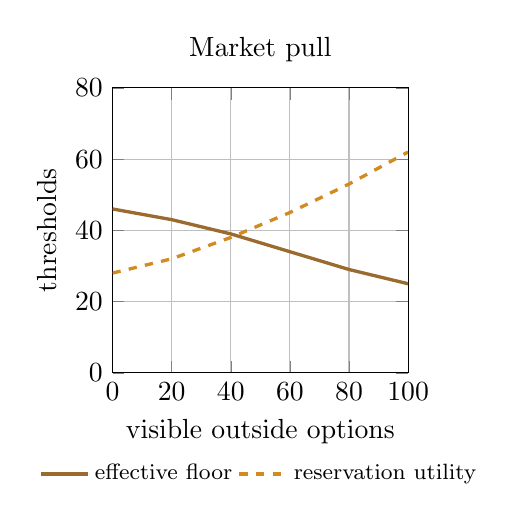
\begin{tikzpicture}
\begin{axis}[
  width=.44\linewidth,
  height=5.2cm,
  xlabel={visible outside options},
  ylabel={thresholds},
  ymin=0,ymax=80,
  xmin=0,xmax=100,
  grid=both,
  title={Market pull},
  legend style={at={(0.5,-0.28)},anchor=north,draw=none,fill=none,font=\footnotesize},
  legend columns=2,
]
\addplot[very thick,floorbrown] coordinates {(0,46) (20,43) (40,39) (60,34) (80,29) (100,25)};
\addplot[very thick,riskorange,dashed] coordinates {(0,28) (20,32) (40,38) (60,45) (80,53) (100,62)};
\legend{effective floor,reservation utility}
\end{axis}
\end{tikzpicture}
\caption{Two sliders explain a lot. Trust controls whether care is received as care. Market abundance can lower the effective floor while raising reservation utility, which narrows the safe zone.}
\label{fig:trust-market}
\end{figure}

\section{Operationalization}
The paper's primitives can be measured or approximated. Robust concern maps to compassionate love and willingness-to-sacrifice scales \citep{sprecher2005,rusbult1998}. Trust maps to attachment and repair dynamics \citep{mikulincer2007,gottman1999}. Identification maps to Inclusion of Other in Self and ``we'' language \citep{aron1992,pennebaker2011}. Accurate attention maps to empathic accuracy and love-map tasks \citep{ickes1997,gottman1999}. Market state maps to perceived alternatives, dating pool, and reservation utility \citep{rusbult1998,rosenfeld2019}. Giving can be approximated with observed care behaviors, daily diary reports of effort, costly sacrifice, and partner-specific behavioral logs. Translation loss can be estimated by comparing what one partner reports giving with what the other reports receiving in the same time window. Genuineness is hardest; it requires consistency across monitored and unmonitored contexts, predictive accuracy of partner state, and low instrumental distortion. Relationship-ending risk can be approximated from breakup ideation, commitment instability, perceived alternatives, chronic unresolved conflict, and the slope of stay-intention as $L(t)$ falls below $R(t)$.

The accompanying dashboard is therefore not a clinical instrument. It is an intuition machine: a way to inspect how assumptions about care, trust, floors, anti-love, outside options, and imbalance interact.

\section{Convergence Across Traditions}
The model is now in place; the literature explains why these variables are not arbitrary. Psychology supplies the dynamics of attachment, passion, repair, and individual differences. Philosophy supplies the normative boundary between love, fantasy, manipulation, and mere utility. Economics supplies search, outside options, bargaining, commitment, and deadweight loss.

\subsection{Psychology}
Sternberg's triangular theory distinguishes intimacy, passion, and commitment \citep{sternberg1986,sternberg1996}. Lee's love styles and the Love Attitudes Scale treat different people as having different priors over which channels count as love \citep{lee1973,hendrick1986}. Attachment theory explains variation in the trust gate: secure partners recover trust more easily, anxious partners register threat more sharply, and avoidant partners cap the gate lower \citep{bowlby1969,ainsworth1978,hazan1987,bartholomew1991,mikulincer2007}. Hatfield and Rapson's passionate/companionate distinction maps onto changes in weight concentration and floor stability \citep{hatfield1978,berscheid2010}. Gottman's work treats micro-interactions as bids and repairs that change trust over time \citep{gottman1999,gottman2011}. Fisher, Brown, Aron, and Carter explain why romantic love is not just intense friendship: attraction and attachment recruit partially distinct neurobiological systems \citep{fisher1998,aron2005,acevedo2012,carter1998}. Aron's self-expansion model explains reflexive weight update: being loved well changes the self that receives love \citep{aron1986,aron2022}. Fredrickson's positivity resonance gives the seconds-long version of the same process \citep{fredrickson2013}. Johnson's emotionally focused therapy shows why trust dominates under stress \citep{johnson2019}. Perel's desire-security tension explains why some weights are antagonistic rather than merely additive \citep{perel2006}. Rusbult's investment model supplies the bridge to reservation utility and outside options \citep{rusbult1980,rusbult1998}.

\subsection{Philosophy}
Plato's ladder already separates attraction to a beautiful particular from a more general pull toward the good \citep{plato1997}. Aristotle and Aquinas frame love as willing the good of the other for the other's sake \citep{aristotle1999,aquinas1947}. Augustine and Kierkegaard make love partly a question of ordering and commitment rather than merely appetite \citep{augustine1991,kierkegaard1995}. Spinoza and Nussbaum show why love is still affective and evaluative, not just moral law \citep{spinoza1994,nussbaum2001}. Fromm and hooks define love as active care, responsibility, respect, knowledge, commitment, and growth \citep{fromm1956,hooks2000}. Frankfurt gives disinterested concern, personal particularity, identification, and volitional necessity \citep{frankfurt2004}. Murdoch and Weil add accurate attention: love must see the other as real rather than as a projection \citep{murdoch1970,weil1951}. Velleman, Kolodny, Nozick, and Helm clarify why love is not replaceable by a list of attractive properties; it depends on the person, the relationship, and the shared evaluative perspective \citep{velleman1999,kolodny2003,nozick1989,helm2010}. Badiou makes romantic love a construction over time: a scene of Two sustained by fidelity to an encounter \citep{badiou2012}.

\subsection{Economics}
Becker's family economics, search theory, bargaining models, and Rusbult's psychological investment model all point to outside options and reservation utility \citep{becker1973,becker1981,mortensen1986,manser1980,mcelroy1981}. Sex-ratio work shows that market scarcity changes dyadic power and commitment terms \citep{guttentag1983,angrist2002}. Lundberg and Pollak's bargaining models explain why within-relationship threat points can matter as much as divorce itself \citep{lundberg1993,lundberg1996}. Frank's account of emotions as commitment devices explains why love can rationally include a floor that resists market updating \citep{frank1988}. Costly signaling and mate-choice work explain why some acts of care carry more information than cheap displays \citep{zahavi1975,miller2000}. Repeated-game cooperation, loss aversion, sunk costs, and endowment effects explain why positive and negative interactions do not cancel one-for-one \citep{axelrod1984,kahneman1979,thaler1980}. Dating markets and choice overload alter the visible distribution of alternatives, thereby changing both thresholds and weights \citep{rosenfeld2019,pronk2020}. Optimal stopping gives the formal reason that settling can be rational even when it is emotionally uncomfortable \citep{gilbert1966,bearden2006}.

\section{Limitations}
The update rule $f$ is underdetermined and likely heterogeneous across attachment styles and cultures. The pure-care policy is an idealization. Self-report can be distorted by defensiveness, hope, or fear. The same event may count differently across partners, and some anti-love events should be treated as categorical harms rather than smooth penalties. Finally, the model can describe stable dyads that are not flourishing dyads; ethical interpretation still matters.

\section{Conclusion}
Love is the operation of a reflexive, trust-gated, floor-anchored care function that tracks the genuine flourishing of an accurately perceived particular other across time, embedded in a market of alternatives whose pull the floor commitment is designed to resist. The receiving curve tells us how loved someone feels; the giving curve tells us how much care they send outward; the translation between them tells us whether the relationship is actually communicating love. Relationship-ending risk is the shadow variable: not the opposite of love, but the undesirable probability pressure that appears when love, trust, floor, giving, receiving, and reciprocity no longer stabilize the dyad. Romantic love is that structure plus eros, pair-bonding, negotiated exclusivity, and the ongoing construction of a shared world.

\begin{thebibliography}{99}

\bibitem[Sternberg(1986)]{sternberg1986}
Sternberg, R. J. (1986).
\newblock A triangular theory of love.
\newblock \emph{Psychological Review}, 93(2), 119--135.

\bibitem[Bowlby(1969)]{bowlby1969}
Bowlby, J. (1969).
\newblock \emph{Attachment and Loss}.
\newblock Basic Books.

\bibitem[Hazan and Shaver(1987)]{hazan1987}
Hazan, C., and Shaver, P. (1987).
\newblock Romantic love conceptualized as an attachment process.
\newblock \emph{Journal of Personality and Social Psychology}, 52(3), 511--524.

\bibitem[Bartholomew and Horowitz(1991)]{bartholomew1991}
Bartholomew, K., and Horowitz, L. M. (1991).
\newblock Attachment styles among young adults.
\newblock \emph{Journal of Personality and Social Psychology}, 61(2), 226--244.

\bibitem[Hatfield and Walster(1978)]{hatfield1978}
Hatfield, E., and Walster, G. W. (1978).
\newblock \emph{A New Look at Love}.
\newblock Addison-Wesley.

\bibitem[Gottman(1999)]{gottman1999}
Gottman, J. M. (1999).
\newblock \emph{The Seven Principles for Making Marriage Work}.
\newblock Crown.

\bibitem[Aron and Aron(1986)]{aron1986}
Aron, A., and Aron, E. N. (1986).
\newblock \emph{Love and the Expansion of Self}.
\newblock Hemisphere.

\bibitem[Rusbult(1980)]{rusbult1980}
Rusbult, C. E. (1980).
\newblock Commitment and satisfaction in romantic associations.
\newblock \emph{Journal of Experimental Social Psychology}, 16(2), 172--186.

\bibitem[Rusbult et~al.(1998)]{rusbult1998}
Rusbult, C. E., Martz, J. M., and Agnew, C. R. (1998).
\newblock The Investment Model Scale.
\newblock \emph{Personal Relationships}, 5(4), 357--387.

\bibitem[Aristotle(1999)]{aristotle1999}
Aristotle. (1999).
\newblock \emph{Nicomachean Ethics}.
\newblock Hackett.

\bibitem[Aquinas(1947)]{aquinas1947}
Aquinas, T. (1947).
\newblock \emph{Summa Theologica}.
\newblock Benziger Brothers.

\bibitem[Frankfurt(2004)]{frankfurt2004}
Frankfurt, H. G. (2004).
\newblock \emph{The Reasons of Love}.
\newblock Princeton University Press.

\bibitem[Murdoch(1970)]{murdoch1970}
Murdoch, I. (1970).
\newblock \emph{The Sovereignty of Good}.
\newblock Routledge.

\bibitem[Weil(1951)]{weil1951}
Weil, S. (1951).
\newblock \emph{Waiting for God}.
\newblock Harper.

\bibitem[Nozick(1989)]{nozick1989}
Nozick, R. (1989).
\newblock \emph{The Examined Life}.
\newblock Simon and Schuster.

\bibitem[Helm(2010)]{helm2010}
Helm, B. W. (2010).
\newblock \emph{Love, Friendship, and the Self}.
\newblock Oxford University Press.

\bibitem[Badiou(2012)]{badiou2012}
Badiou, A. (2012).
\newblock \emph{In Praise of Love}.
\newblock The New Press.

\bibitem[Becker(1981)]{becker1981}
Becker, G. S. (1981).
\newblock \emph{A Treatise on the Family}.
\newblock Harvard University Press.

\bibitem[Manser and Brown(1980)]{manser1980}
Manser, M., and Brown, M. (1980).
\newblock Marriage and household decision-making.
\newblock \emph{International Economic Review}, 21(1), 31--44.

\bibitem[McElroy and Horney(1981)]{mcelroy1981}
McElroy, M. B., and Horney, M. J. (1981).
\newblock Nash-bargained household decisions.
\newblock \emph{International Economic Review}, 22(2), 333--349.

\bibitem[Frank(1988)]{frank1988}
Frank, R. H. (1988).
\newblock \emph{Passions Within Reason}.
\newblock W. W. Norton.

\bibitem[Pronk and Denissen(2020)]{pronk2020}
Pronk, T. M., and Denissen, J. J. A. (2020).
\newblock A rejection mind-set.
\newblock \emph{Social Psychological and Personality Science}, 11(3), 388--396.

\bibitem[Rosenfeld et~al.(2019)]{rosenfeld2019}
Rosenfeld, M. J., Thomas, R. J., and Hausen, S. (2019).
\newblock Disintermediating your friends.
\newblock \emph{Proceedings of the National Academy of Sciences}, 116(36), 17753--17758.

\bibitem[Sternberg(1996)]{sternberg1996}
Sternberg, R. J. (1996).
\newblock Love as a story.
\newblock \emph{Personal Relationships}, 3(1), 59--79.

\bibitem[Lee(1973)]{lee1973}
Lee, J. A. (1973).
\newblock \emph{The Colours of Love}.
\newblock New Press.

\bibitem[Hendrick and Hendrick(1986)]{hendrick1986}
Hendrick, C., and Hendrick, S. S. (1986).
\newblock A theory and method of love.
\newblock \emph{Journal of Personality and Social Psychology}, 50(2), 392--402.

\bibitem[Ainsworth et~al.(1978)]{ainsworth1978}
Ainsworth, M. D. S., Blehar, M. C., Waters, E., and Wall, S. (1978).
\newblock \emph{Patterns of Attachment}.
\newblock Erlbaum.

\bibitem[Mikulincer and Shaver(2007)]{mikulincer2007}
Mikulincer, M., and Shaver, P. R. (2007).
\newblock \emph{Attachment in Adulthood}.
\newblock Guilford Press.

\bibitem[Berscheid(2010)]{berscheid2010}
Berscheid, E. (2010).
\newblock Love in the fourth dimension.
\newblock \emph{Annual Review of Psychology}, 61, 1--25.

\bibitem[Gottman(2011)]{gottman2011}
Gottman, J. M. (2011).
\newblock \emph{The Science of Trust}.
\newblock W. W. Norton.

\bibitem[Fisher(1998)]{fisher1998}
Fisher, H. E. (1998).
\newblock Lust, attraction, and attachment in mammalian reproduction.
\newblock \emph{Human Nature}, 9, 23--52.

\bibitem[Aron et~al.(2005)]{aron2005}
Aron, A., Fisher, H., Mashek, D. J., Strong, G., Li, H., and Brown, L. L. (2005).
\newblock Reward, motivation, and emotion systems associated with early-stage intense romantic love.
\newblock \emph{Journal of Neurophysiology}, 94(1), 327--337.

\bibitem[Acevedo et~al.(2012)]{acevedo2012}
Acevedo, B. P., Aron, A., Fisher, H. E., and Brown, L. L. (2012).
\newblock Neural correlates of long-term intense romantic love.
\newblock \emph{Social Cognitive and Affective Neuroscience}, 7(2), 145--159.

\bibitem[Carter(1998)]{carter1998}
Carter, C. S. (1998).
\newblock Neuroendocrine perspectives on social attachment and love.
\newblock \emph{Psychoneuroendocrinology}, 23(8), 779--818.

\bibitem[Aron et~al.(2022)]{aron2022}
Aron, A., Lewandowski, G. W., Branand, B., Mashek, D., and Aron, E. N. (2022).
\newblock Self-expansion motivation and inclusion of others in self.
\newblock \emph{Journal of Social and Personal Relationships}, 39(12), 3823--3852.

\bibitem[Fredrickson(2013)]{fredrickson2013}
Fredrickson, B. L. (2013).
\newblock \emph{Love 2.0}.
\newblock Hudson Street Press.

\bibitem[Johnson(2019)]{johnson2019}
Johnson, S. M. (2019).
\newblock \emph{Attachment Theory in Practice}.
\newblock Guilford Press.

\bibitem[Perel(2006)]{perel2006}
Perel, E. (2006).
\newblock \emph{Mating in Captivity}.
\newblock Harper.

\bibitem[Plato(1997)]{plato1997}
Plato. (1997).
\newblock Symposium.
\newblock In J. M. Cooper (Ed.), \emph{Plato: Complete Works}. Hackett.

\bibitem[Augustine(1991)]{augustine1991}
Augustine. (1991).
\newblock \emph{Confessions}.
\newblock Oxford University Press.

\bibitem[Kierkegaard(1995)]{kierkegaard1995}
Kierkegaard, S. (1995).
\newblock \emph{Works of Love}.
\newblock Princeton University Press.

\bibitem[Spinoza(1994)]{spinoza1994}
Spinoza, B. (1994).
\newblock \emph{A Spinoza Reader}.
\newblock Princeton University Press.

\bibitem[Nussbaum(2001)]{nussbaum2001}
Nussbaum, M. C. (2001).
\newblock \emph{Upheavals of Thought}.
\newblock Cambridge University Press.

\bibitem[Fromm(1956)]{fromm1956}
Fromm, E. (1956).
\newblock \emph{The Art of Loving}.
\newblock Harper and Row.

\bibitem[hooks(2000)]{hooks2000}
hooks, b. (2000).
\newblock \emph{All About Love}.
\newblock William Morrow.

\bibitem[Velleman(1999)]{velleman1999}
Velleman, J. D. (1999).
\newblock Love as a moral emotion.
\newblock \emph{Ethics}, 109(2), 338--374.

\bibitem[Kolodny(2003)]{kolodny2003}
Kolodny, N. (2003).
\newblock Love as valuing a relationship.
\newblock \emph{The Philosophical Review}, 112(2), 135--189.

\bibitem[Becker(1973)]{becker1973}
Becker, G. S. (1973).
\newblock A theory of marriage: Part I.
\newblock \emph{Journal of Political Economy}, 81(4), 813--846.

\bibitem[Mortensen(1986)]{mortensen1986}
Mortensen, D. T. (1986).
\newblock Job search and labor market analysis.
\newblock In O. Ashenfelter and R. Layard (Eds.), \emph{Handbook of Labor Economics}. Elsevier.

\bibitem[Guttentag and Secord(1983)]{guttentag1983}
Guttentag, M., and Secord, P. F. (1983).
\newblock \emph{Too Many Women?}
\newblock Sage.

\bibitem[Angrist(2002)]{angrist2002}
Angrist, J. (2002).
\newblock How do sex ratios affect marriage and labor markets?
\newblock \emph{Quarterly Journal of Economics}, 117(3), 997--1038.

\bibitem[Lundberg and Pollak(1993)]{lundberg1993}
Lundberg, S., and Pollak, R. A. (1993).
\newblock Separate spheres bargaining and the marriage market.
\newblock \emph{Journal of Political Economy}, 101(6), 988--1010.

\bibitem[Lundberg and Pollak(1996)]{lundberg1996}
Lundberg, S., and Pollak, R. A. (1996).
\newblock Bargaining and distribution in marriage.
\newblock \emph{Journal of Economic Perspectives}, 10(4), 139--158.

\bibitem[Zahavi(1975)]{zahavi1975}
Zahavi, A. (1975).
\newblock Mate selection: A selection for a handicap.
\newblock \emph{Journal of Theoretical Biology}, 53(1), 205--214.

\bibitem[Miller(2000)]{miller2000}
Miller, G. (2000).
\newblock \emph{The Mating Mind}.
\newblock Doubleday.

\bibitem[Axelrod(1984)]{axelrod1984}
Axelrod, R. (1984).
\newblock \emph{The Evolution of Cooperation}.
\newblock Basic Books.

\bibitem[Kahneman and Tversky(1979)]{kahneman1979}
Kahneman, D., and Tversky, A. (1979).
\newblock Prospect theory.
\newblock \emph{Econometrica}, 47(2), 263--291.

\bibitem[Thaler(1980)]{thaler1980}
Thaler, R. (1980).
\newblock Toward a positive theory of consumer choice.
\newblock \emph{Journal of Economic Behavior and Organization}, 1(1), 39--60.

\bibitem[Gilbert and Mosteller(1966)]{gilbert1966}
Gilbert, J. P., and Mosteller, F. (1966).
\newblock Recognizing the maximum of a sequence.
\newblock \emph{Journal of the American Statistical Association}, 61(313), 35--73.

\bibitem[Bearden et~al.(2006)]{bearden2006}
Bearden, J. N., Rapoport, A., and Murphy, R. O. (2006).
\newblock Sequential observation and selection with rank-dependent payoffs.
\newblock \emph{Management Science}, 52(9), 1437--1449.

\bibitem[Sprecher and Fehr(2005)]{sprecher2005}
Sprecher, S., and Fehr, B. (2005).
\newblock Compassionate love for close others and humanity.
\newblock \emph{Journal of Social and Personal Relationships}, 22(5), 629--651.

\bibitem[Aron et~al.(1992)]{aron1992}
Aron, A., Aron, E. N., and Smollan, D. (1992).
\newblock Inclusion of Other in the Self Scale and the structure of interpersonal closeness.
\newblock \emph{Journal of Personality and Social Psychology}, 63(4), 596--612.

\bibitem[Pennebaker(2011)]{pennebaker2011}
Pennebaker, J. W. (2011).
\newblock \emph{The Secret Life of Pronouns}.
\newblock Bloomsbury Press.

\bibitem[Ickes(1997)]{ickes1997}
Ickes, W. (Ed.). (1997).
\newblock \emph{Empathic Accuracy}.
\newblock Guilford Press.

\end{thebibliography}

\end{document}
